\documentclass[french]{article}
\usepackage[T1]{fontenc}
\usepackage[utf8]{inputenc}
\usepackage{lmodern}
\usepackage[a4paper]{geometry}
\usepackage{babel}
\usepackage{graphicx}

\begin{document}
	\title{Nuages de points et modélisation 3D\\
		TP 6 : Modelling
	}
	\author{Marius Dufraisse}
	\date{}
	
	\maketitle
	
	\paragraph{Question 1.}
	The prominent plane represents the floor, it contains 135366 points.
	
	\paragraph{Question 2.}
	The probability to sample 3 points in this plane is roughly $\left(\frac{135366}{412756}\right)^3\approx0.0353$ thus the probability of not finding this plane when drawing $N$ times is $(1-0.0353)^N$. Thus to find this plane with probability more than 99\% we need $N$ to be such that $(1-0.0353)^N < 0.01$ that is $N > \frac{\log 0.01}{\log(1-0.0353)}\approx 128 $. The floor can be found 99\% of the time by drawing only 128 planes at random.
	
	\paragraph{Question 3.}
	The results obtained when applying RANSAC multiple times are displayed in Figure \ref{fig:q3}. The results are not satisfying, I assume this comes from bad plane candidates can still contain lot of points across the range of the point cloud.
	
	\begin{figure}[h!]
		\centering
		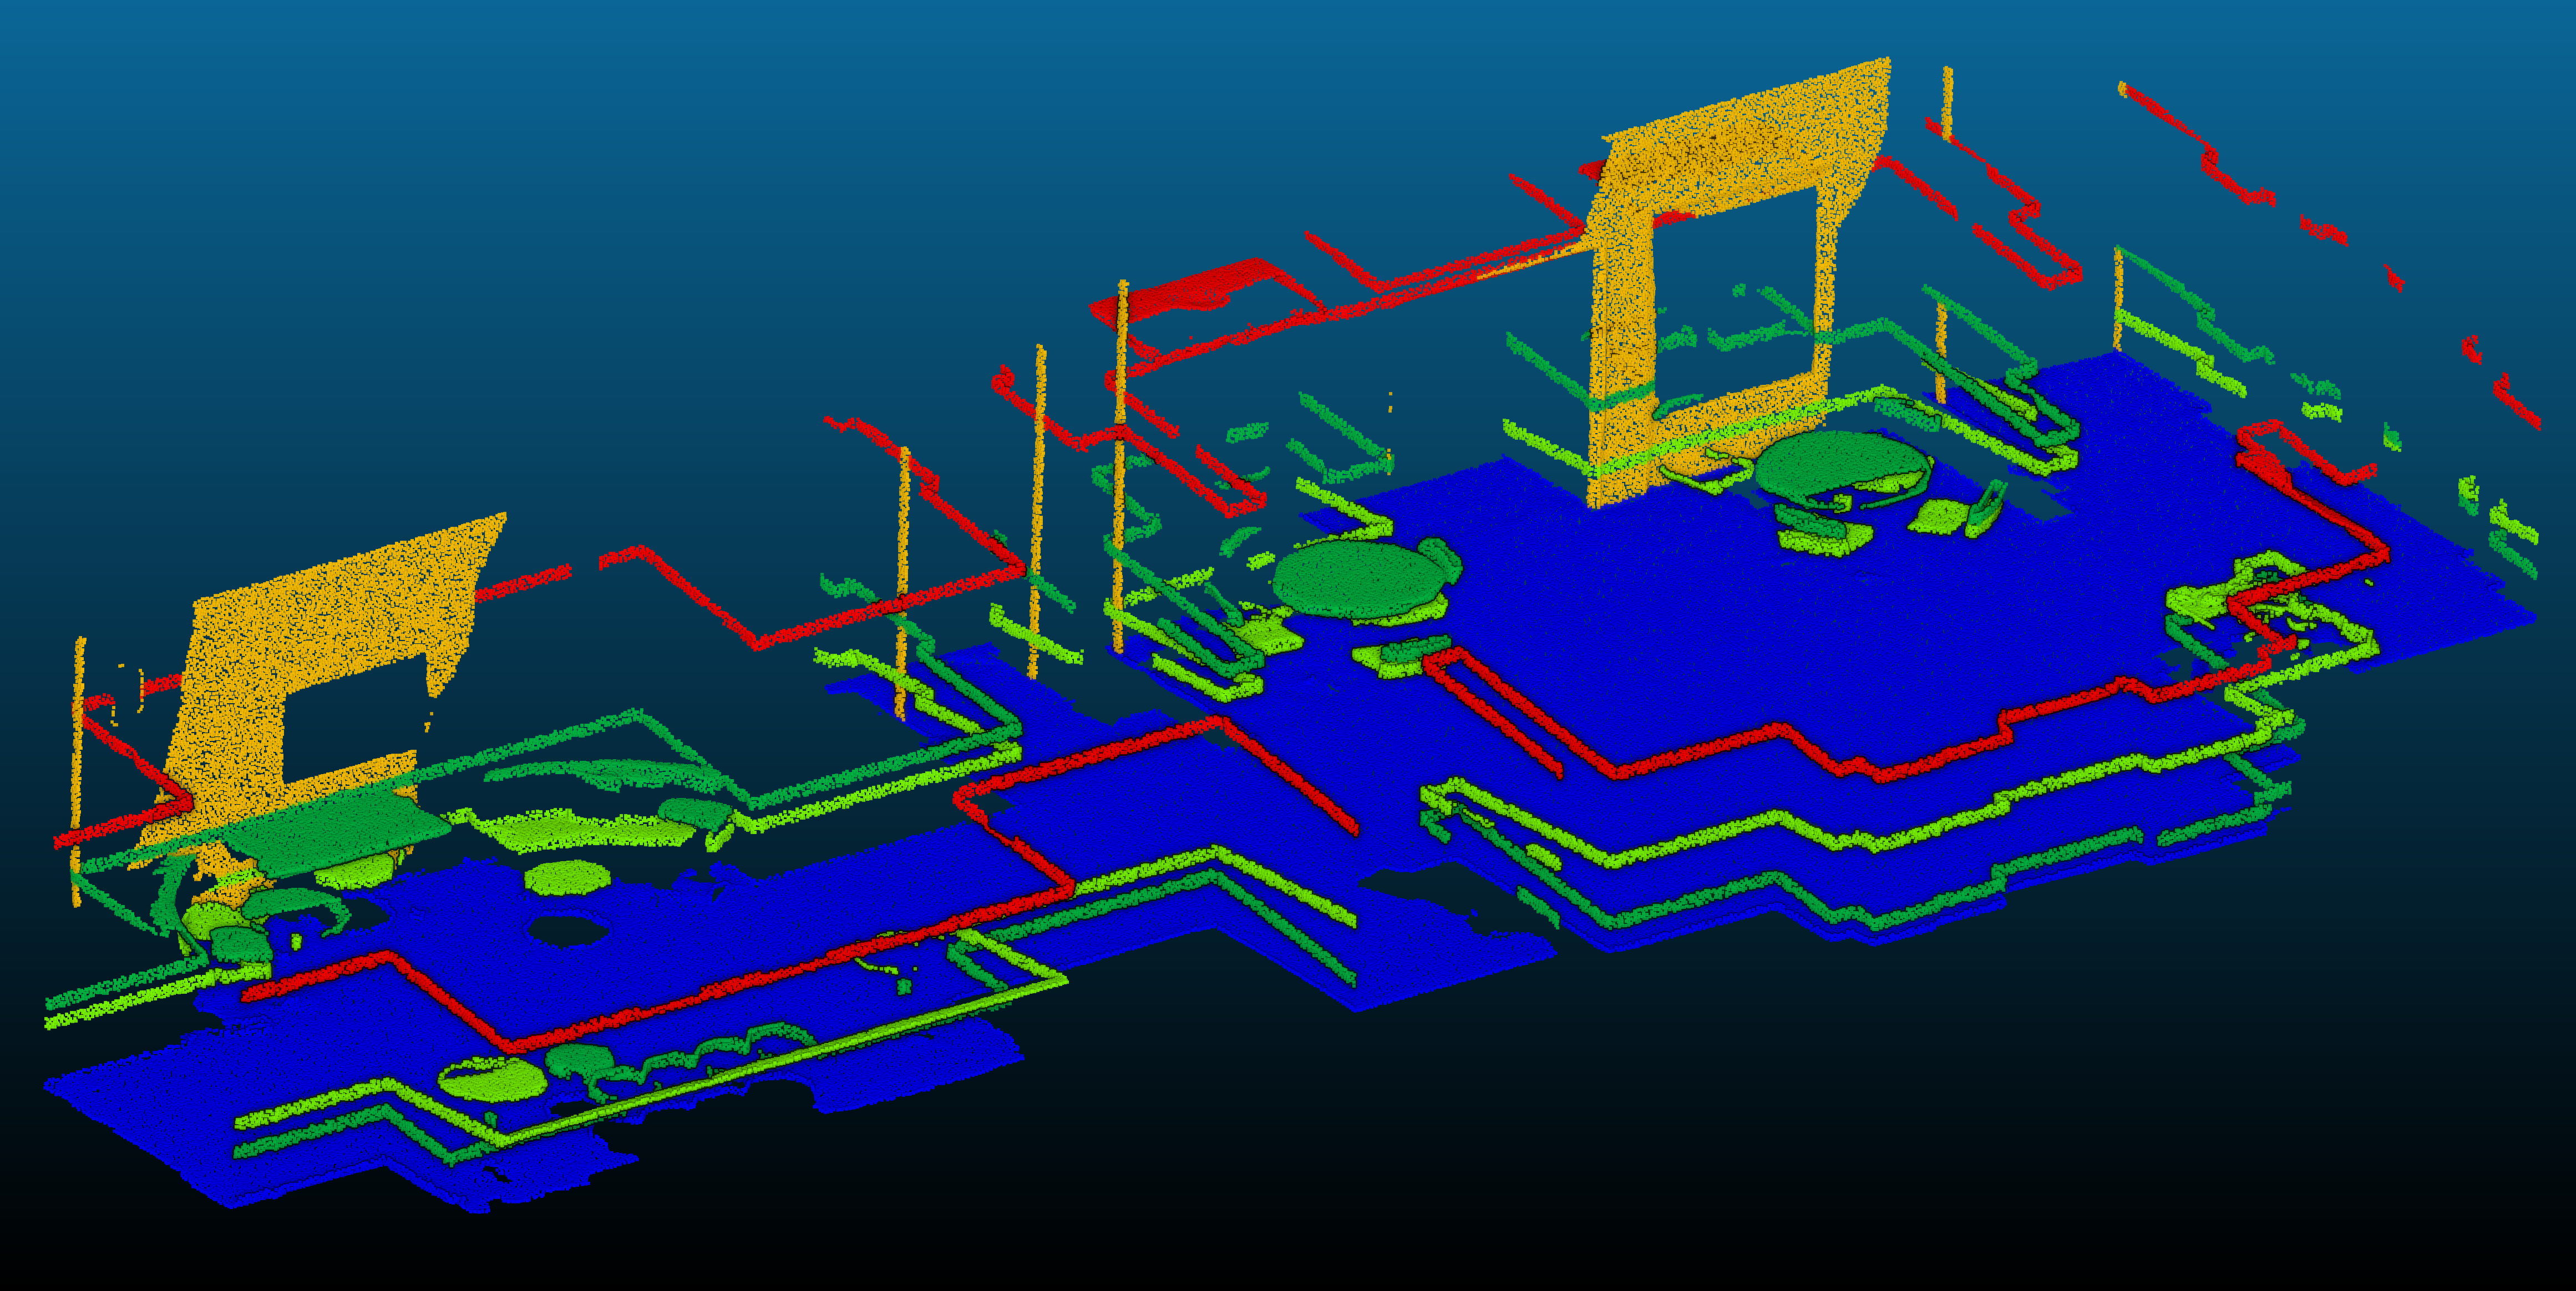
\includegraphics[width=\linewidth]{q3.png}
		\caption{Results obtained when applying RANSAC multiple times.}
		\label{fig:q3}
	\end{figure}
	
	\paragraph{Question 4.}
	If the angle threshold is too high points on planes close to the main one are added to the result, if it is too small, points will be missing near the edges of the plan.
	
	The threshold in \texttt{region\textunderscore{}criterion} can be chosen within a large range of values without impacting the result.
	
	The threshold need to be high enough otherwise the computation time will be increased a lot and too many points will be added to the plane.
	
	If the growing radius is too big, the algorithm is slower and produces worst results with too many points added to the plan. If it is too small there will be some points missing in the result.
	
	\paragraph{Question 5.} 
	In order to increase the chances of finding a plane we can take a seed with a high planarity as it is more likely to be part of a plan.
	
	
	\paragraph{Question 6.} The results obtained with the region growing method can be seen in Figure \ref{fig:q6}.
	
	Region growing is as fast as RANSAC (when RANSAC has enough iterations to exceed the bound on draws required to get good planes 99\% of the time) but the results are much better. Region Growing tends to split planes in two (for instance above the central arch) whereas RANSAC would extend them across the point cloud.
	
	\begin{figure}[h!]
		\centering
		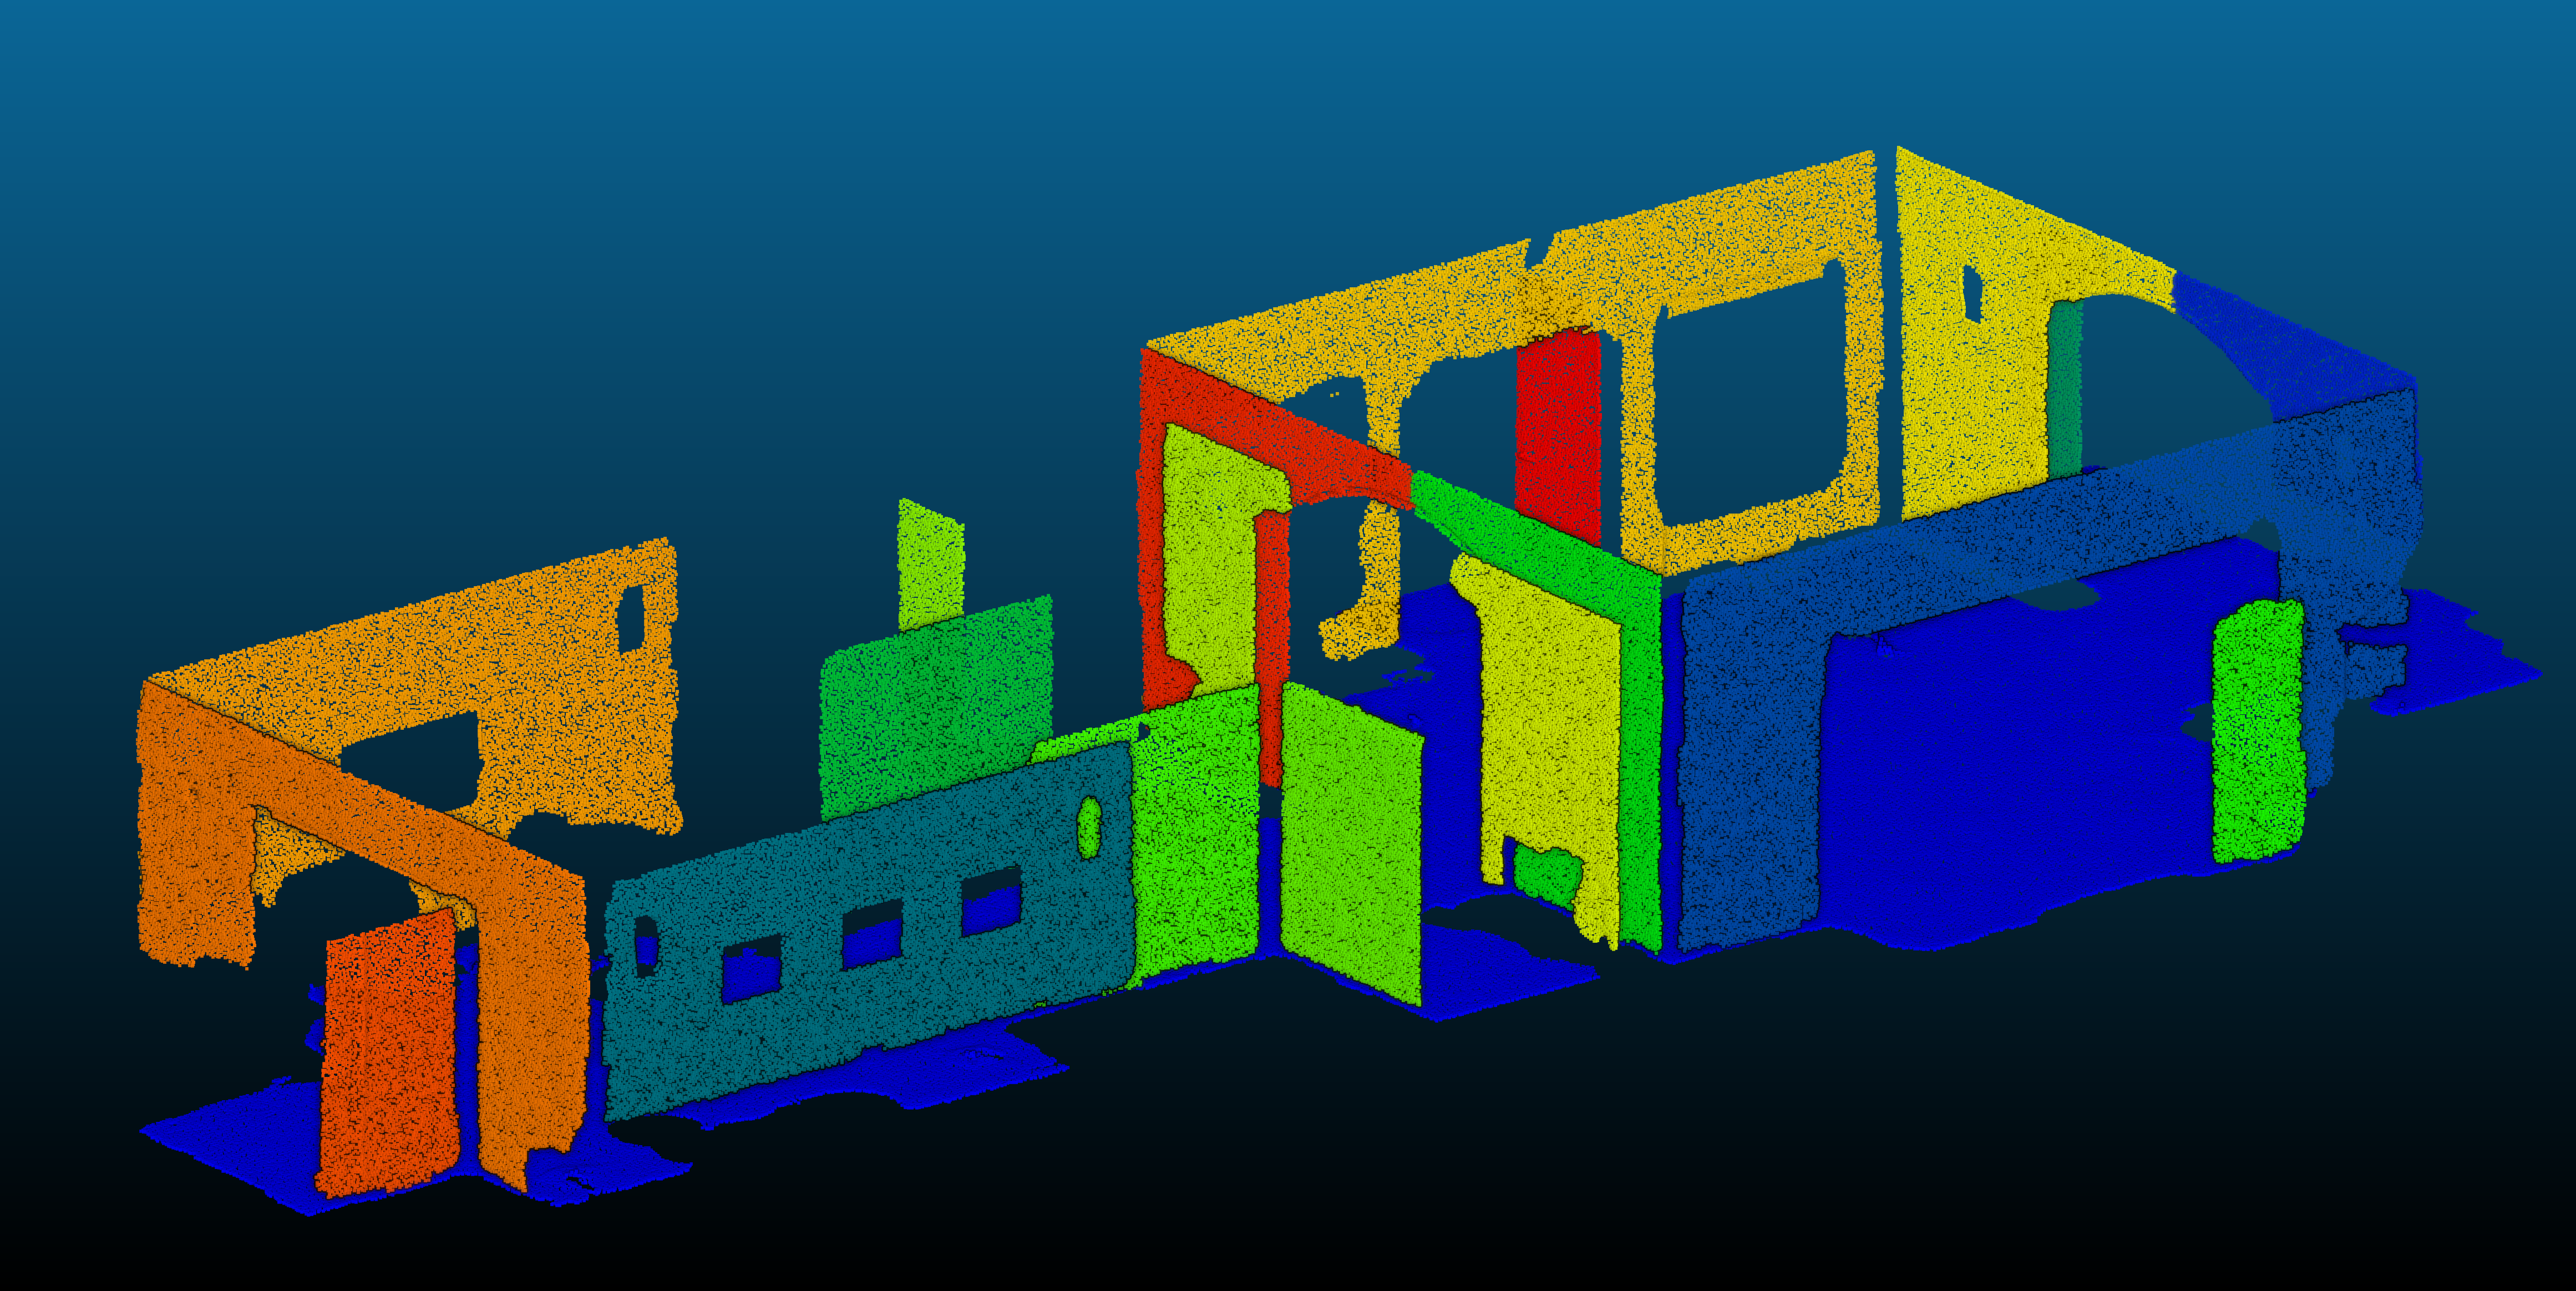
\includegraphics[width=\linewidth]{q6-20.png}
		\caption{Results obtained when applying the region growing algorithm to find 20 planes.}
		\label{fig:q6}
	\end{figure}
	
\end{document}

